		\documentclass[landscape,final,a0paper,fontscale=0.285]{baposter}
		
		\usepackage{calc}
		\usepackage{graphicx}
		\usepackage{amsmath}
		\usepackage{amssymb}
		\usepackage{relsize}
		\usepackage{multirow}
		\usepackage{rotating}
		\usepackage{bm}
		\usepackage{url}
		\usepackage{color}
		\usepackage{colortbl}

		
		\usepackage{graphicx}
		\usepackage{multicol}
		\usepackage{picture}
		
		%\usepackage{times}
		%\usepackage{helvet}
		%\usepackage{bookman}
		\usepackage{palatino}
		
\usepackage{alltt}
\usepackage{verbatim}

		\newcommand{\captionfont}{\footnotesize}
		
		\graphicspath{{images/}{../images/}}
		\usetikzlibrary{calc}
		
		\newcommand{\SET}[1]  {\ensuremath{\mathcal{#1}}}
		\newcommand{\MAT}[1]  {\ensuremath{\boldsymbol{#1}}}
		\newcommand{\VEC}[1]  {\ensuremath{\boldsymbol{#1}}}
		\newcommand{\Video}{\SET{V}}
		\newcommand{\video}{\VEC{f}}
		\newcommand{\track}{x}
		\newcommand{\Track}{\SET T}
		\newcommand{\LMs}{\SET L}
		\newcommand{\lm}{l}
		\newcommand{\PosE}{\SET P}
		\newcommand{\posE}{\VEC p}
		\newcommand{\negE}{\VEC n}
		\newcommand{\NegE}{\SET N}
		\newcommand{\Occluded}{\SET O}
		\newcommand{\occluded}{o}

		\newcommand{\eat}[1]{}
		
		%%%%%%%%%%%%%%%%%%%%%%%%%%%%%%%%%%%%%%%%%%%%%%%%%%%%%%%%%%%%%%%%%%%%%%%%%%%%%%%%
		%%%% Some math symbols used in the text
		%%%%%%%%%%%%%%%%%%%%%%%%%%%%%%%%%%%%%%%%%%%%%%%%%%%%%%%%%%%%%%%%%%%%%%%%%%%%%%%%
		
		%%%%%%%%%%%%%%%%%%%%%%%%%%%%%%%%%%%%%%%%%%%%%%%%%%%%%%%%%%%%%%%%%%%%%%%%%%%%%%%%
		% Multicol Settings
		%%%%%%%%%%%%%%%%%%%%%%%%%%%%%%%%%%%%%%%%%%%%%%%%%%%%%%%%%%%%%%%%%%%%%%%%%%%%%%%%
		\setlength{\columnsep}{1em}
		\setlength{\columnseprule}{0mm}
		
		%%%%%%%%%%%%%%%%%%%%%%%%%%%%%%%%%%%%%%%%%%%%%%%%%%%%%%%%%%%%%%%%%%%%%%%%%%%%%%%%
		% Save space in lists. Use this after the opening of the list
		%%%%%%%%%%%%%%%%%%%%%%%%%%%%%%%%%%%%%%%%%%%%%%%%%%%%%%%%%%%%%%%%%%%%%%%%%%%%%%%%
		\newcommand{\compresslist}{%
		\setlength{\itemsep}{1pt}%
		\setlength{\parskip}{0pt}%
		\setlength{\parsep}{0pt}%
		}
		
		%%%%%%%%%%%%%%%%%%%%%%%%%%%%%%%%%%%%%%%%%%%%%%%%%%%%%%%%%%%%%%%%%%%%%%%%%%%%%%
		%%% Begin of Document
		%%%%%%%%%%%%%%%%%%%%%%%%%%%%%%%%%%%%%%%%%%%%%%%%%%%%%%%%%%%%%%%%%%%%%%%%%%%%%%
		
		\begin{document}
		
		%%%%%%%%%%%%%%%%%%%%%%%%%%%%%%%%%%%%%%%%%%%%%%%%%%%%%%%%%%%%%%%%%%%%%%%%%%%%%%
		%%% Here starts the poster
		%%%---------------------------------------------------------------------------
		%%% Format it to your taste with the options
		%%%%%%%%%%%%%%%%%%%%%%%%%%%%%%%%%%%%%%%%%%%%%%%%%%%%%%%%%%%%%%%%%%%%%%%%%%%%%%
		% Define some colors
		
		%\definecolor{lightblue}{cmyk}{0.83,0.24,0,0.12}
		\definecolor{lightblue}{rgb}{0.145,0.6666,1}
		
		% Draw a video
		\newlength{\FSZ}
		\newcommand{\drawvideo}[3]{% [0 0.25 0.5 0.75 1 1.25 1.5]
		   \noindent\pgfmathsetlength{\FSZ}{\linewidth/#2}
		   \begin{tikzpicture}[outer sep=0pt,inner sep=0pt,x=\FSZ,y=\FSZ]
		   \draw[color=lightblue!50!black] (0,0) node[outer sep=0pt,inner sep=0pt,text width=\linewidth,minimum height=0] (video) {\noindent#3};
		   \path [fill=lightblue!50!black,line width=0pt] 
		     (video.north west) rectangle ([yshift=\FSZ] video.north east) 
		    \foreach \x in {1,2,...,#2} {
		      {[rounded corners=0.6] ($(video.north west)+(-0.7,0.8)+(\x,0)$) rectangle +(0.4,-0.6)}
		    }
		;
		   \path [fill=lightblue!50!black,line width=0pt] 
		     ([yshift=-1\FSZ] video.south west) rectangle (video.south east) 
		    \foreach \x in {1,2,...,#2} {
		      {[rounded corners=0.6] ($(video.south west)+(-0.7,-0.2)+(\x,0)$) rectangle +(0.4,-0.6)}
		    }
		;
		   \foreach \x in {1,...,#1} {
		     \draw[color=lightblue!50!black] ([xshift=\x\linewidth/#1] video.north west) -- ([xshift=\x\linewidth/#1] video.south west);
		   }
		   \foreach \x in {0,#1} {
		     \draw[color=lightblue!50!black] ([xshift=\x\linewidth/#1,yshift=1\FSZ] video.north west) -- ([xshift=\x\linewidth/#1,yshift=-1\FSZ] video.south west);
		   }
		   \end{tikzpicture}
		}
		
		\hyphenation{resolution occlusions}
		%%
		\begin{poster}%
		  % Poster Options
		  {
		  % Show grid to help with alignment
		  grid=false,
		  % Column spacing
		  colspacing=0.5em,
		  %colspacing=1em,
		  % Color style
		  bgColorOne=white,
		  bgColorTwo=white,
		  borderColor=lightblue,
		  headerColorOne=black,
		  headerColorTwo=lightblue,
		  headerFontColor=white,
		  boxColorOne=white,
		  boxColorTwo=lightblue,
		  % Format of textbox
		  textborder=roundedleft,
		  % Format of text header
		  eyecatcher=false,
		  headerborder=closed,
		  headerheight=0.110\textheight,
		  %headerheight=0.090\textheight,
		  %headerheight=0.125\textheight,
		%  textfont=\sc, An example of changing the text font
		  headershape=roundedright,
		  headershade=shadelr,
		  headerfont=\Large\bf\textsc, %Sans Serif
		  textfont={\setlength{\parindent}{1.2em}},
		  %textfont={\setlength{\parindent}{1.5em}},
		  boxshade=plain,
		%  background=shade-tb,
		  background=plain,
		  linewidth=2pt
		  }
		  % Eye Catcher
		  {\includegraphics[height=3em]{images/graph_occluded.pdf}} 
		  % Title
		  {\vspace*{2pt}\bf{\underline{MADden: Query-Driven Statistical Text Analytics}}\vspace{-0.10em}}
		  % Authors
		  {\textsc{ Christan Grant$^{\S}$, Joir-dan Gumbs$^{\S}$, Kun Li$^{\S}$, Daisy Zhe Wang$^{\S}$| George Chitouras$^{\dagger}$\\    
		                    {$^{\S}$\textit{Database Research Center, CISE, University of Florida} | $^{\dagger}$\textit{Greenplum EMC} }}\\
		             {\textit{\textcolor{blue} {\{cgrant, jgumbs, kli, daisyw\} @cise.ufl.edu}}| \textit{george.chitouras@emc.com}  }}
		  % University logo
		  {% The makebox allows the title to flow into the logo, this is a hack because of the L shaped logo.
		    
\includegraphics[height=6.0em, width=18.0em]{logo/UF_Signature_Themeline.pdf}
		    
\includegraphics[height=6.0em, width=15.0em]{logo/gp_logo.jpg}
		  }\vspace{-3mm}
		
		%%%%%%%%%%%%%%%%%%%%%%%%%%%%%%%%%%%%%%%%%%%%%%%%%%%%%%%%%%%%%%%%%%%%%%%%%%%%%%
		%%% Now define the boxes that make up the poster
		%%%---------------------------------------------------------------------------
		%%% Each box has a name and can be placed absolutely or relatively.
		%%% The only inconvenience is that you can only specify a relative position 
		%%% towards an already declared box. So if you have a box attached to the 
		%%% bottom, one to the top and a third one which should be in between, you 
		%%% have to specify the top and bottom boxes before you specify the middle 
		%%% box.
		%%%%%%%%%%%%%%%%%%%%%%%%%%%%%%%%%%%%%%%%%%%%%%%%%%%%%%%%%%%%%%%%%%%%%%%%%%%%%%
		    %
		    % A coloured circle useful as a bullet with an adjustably strong filling
		    \newcommand{\colouredcircle}{%
		      \tikz{\useasboundingbox (-0.2em,-0.32em) rectangle(0.2em,0.32em); \draw[draw=black,fill=lightblue,line width=0.03em] (0,0) circle(0.18em);}}
		
		%%%%%%%%%%%%%%%%%%%%%%%%%%%%%%%%%%%%%%%%%%%%%%%%%%%%%%%%%%%%%%%%%%%%%%%%%%%%%%
		  \headerbox{Abstract}{name=myabstract,column=0,row=0}{
		%%%%%%%%%%%%%%%%%%%%%%%%%%%%%%%%%%%%%%%%%%%%%%%%%%%%%%%%%%%%%%%%%%%%%%%%%%%%%%
		  	\newcommand{\compactlist}{\setlength{\itemsep}{0pt} \setlength{\parskip}{0pt} \setlength{\leftskip}{-1em}}
In MADden we demonstrate techniques for in-database statistical text analytics over sports data.
The advantages of this mode is:\\
    1. Ad hoc declarative queries through the SQL interface.\\
    2. Easily import and use external libraries.\\
    3. Scalability of leading algorithms through SQL parallel databases.\\
We describe these principles through MADden.



			}
			
		%%%%%%%%%%%%%%%%%%%%%%%%%%%%%%%%%%%%%%%%%%%%%%%%%%%%%%%%%%%%%%%%%%%%%%%%%%%%%%
		  \headerbox{Data Set}{name=myintroduction,column=0,below=myabstract}{
		%%%%%%%%%%%%%%%%%%%%%%%%%%%%%%%%%%%%%%%%%%%%%%%%%%%%%%%%%%%%%%%%%%%%%%%%%%%%%%
		   \newcommand{\compactlist}{\setlength{\itemsep}{0pt} \setlength{\parskip}{0pt} \setlength{\leftskip}{-1em}}
 
We obtained sports data from the 2011 National Football League (NFL) Season, POS data from CoNLL-2000 and movie review data from Cornell.
\begin{center}
\begin{tabular}{|l|r|r|}
\hline
\textbf{Table} & \textbf{Rows} & \textbf{Size} \\
\hline
Tweets & 23,912,687 & 9,178 MB\\
\hline
NFL Plays & 100,271 & 18 MB \\
\hline
NFL Recaps & 14,151 & 4 MB\\
\hline
Movie Reviews & 2,000 & 12 MB\\
\hline
CoNLL-2000 & 30,000 & 3 MB \\
\hline
\end{tabular}
\end{center}

			}

                %%%%%%%%%%%%%%%%%%%%%%%%%%%%%%%%%%%%%%%%%%%%%%%%%%%%%%%%%%%%%%%%%%%%%%%%%%%%%%
                  \headerbox{Queries}{name=myqueries, column=0,below=myintroduction}{
                %%%%%%%%%%%%%%%%%%%%%%%%%%%%%%%%%%%%%%%%%%%%%%%%%%%%%%%%%%%%%%%%%%%%%%%%%%%%%%
								We can use UDFs and use external libraries to perform computations.
								Here is an example query for part-of-speech tagging:\\
\indent \textit{SELECT term, pos}\\
\indent \textit{FROM postag(<text>)};\\
								Here is a function for named-entity recognition:\\
\indent \textit{SELECT term, tag}\\
\indent \textit{FROM ne\_chunk(<text>);}

}



                %%%%%%%%%%%%%%%%%%%%%%%%%%%%%%%%%%%%%%%%%%%%%%%%%%%%%%%%%%%%%%%%%%%%%%%%%%%%%%
                  \headerbox{Performance Evaluation}{name=myexperiment,column=0,below=myqueries}{
                %%%%%%%%%%%%%%%%%%%%%%%%%%%%%%%%%%%%%%%%%%%%%%%%%%%%%%%%%%%%%%%%%%%%%%%%%%%%%%
                  %       \includegraphics[width=0.85\linewidth]{T-labs-Drawing-1} 
                          \newcommand{\compactlist}{\setlength{\itemsep}{0pt} \setlength{\parskip}{0pt} \setlength{\leftskip}{-1em}}
\begin{center}CRF: \textcolor{green}{Postgres} VS \textcolor{blue}{Greenplum(2 cores)}\\
Text Feature Extraction + Viterbi Inference\end{center}
                                        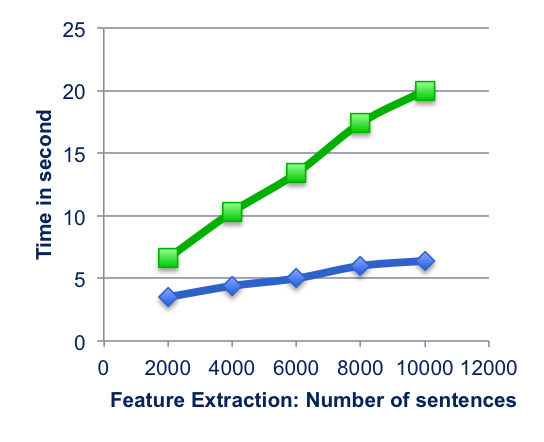
\includegraphics[height=9.9em,width=10em]{images/extraction.png}
                                        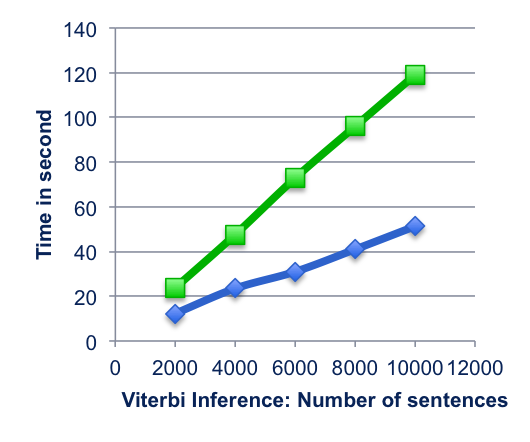
\includegraphics[height=9.9em,width=10em]{images/viterbi.png}

                }

		 		%%%%%%%%%%%%%%%%%%%%%%%%%%%%%%%%%%%%%%%%%%%%%%%%%%%%%%%%%%%%%%%%%%%%%%%%%%%%%%
		  \headerbox{MADlib Text Analytics}{name=myourapproach,column=1,span=3,row=0}{
		  %\headerbox{Parallel Text Feature Extraction}{name=myourapproach,column=1,span=3,row=0}{
		%%%%%%%%%%%%%%%%%%%%%%%%%%%%%%%%%%%%%%%%%%%%%%%%%%%%%%%%%%%%%%%%%%%%%%%%%%%%%%
			
			  \newcommand{\compactlist}{\setlength{\itemsep}{0pt} \setlength{\parskip}{0pt} \setlength{\leftskip}{-1em}}

  \begin{multicols}{2}
\textbf{MADlib} is an open-source library for scalable in-database analytics.
Using Greenplum DB we can take advantage of data-parallel implementations
of mathematical, statistical and machine-learning methods for structured 
and unstructured data. \url{http://github.com/madlib}
\\
\\
\textbf{Available packages} \\
Association Rule Mining $\cdot$
Naive Bayes $\cdot$
Conjugate gradient $\cdot$
Matrix Factorization $\cdot$
\textbf{\textcolor{blue}{Conditional Random Fields}} $\cdot$
KMeans $\cdot$
Linear Regression $\cdot$
Logistic Regression $\cdot$
Statistical and Probabilistic Functions

%We contribute the text analytics package.\\

  \end{multicols}

		
			}
		%%%%%%%%%%%%%%%%%%%%%%%%%%%%%%%%%%%%%%%%%%%%%%%%%%%%%%%%%%%%%%%%%%%%%%%%%%%%%%
		  \headerbox{Parallel Linear-chain CRF Training}{name=myapproxstrmatch,column=1,span=3,below=myourapproach}{
		%%%%%%%%%%%%%%%%%%%%%%%%%%%%%%%%%%%%%%%%%%%%%%%%%%%%%%%%%%%%%%%%%%%%%%%%%%%%%%
			  \newcommand{\compactlist}{\setlength{\itemsep}{0pt} \setlength{\parskip}{0pt} \setlength{\leftskip}{-1em}}
  \begin{multicols}{2}

CRFs are the state of art probabilistic models on a number of real-world tasks including NLP tasks 
such as POS, NER. However CRF training is more computationally expensive due to the expensive 
log-likelihood and gradient vector computation compared with MEMMs and HMMs. We use a Python UDF to drive the computation until the stop criterion is met.
 Within each iteration, we use user-defined
aggregate functions to parallel the computation of the log-likelihood and gradient vector over all documents. At the end of each iteration, the LBFGS optimization is adopted
to update the weight vector.\\
   %\begin{multicols}{2} 
\begin{center}		             
      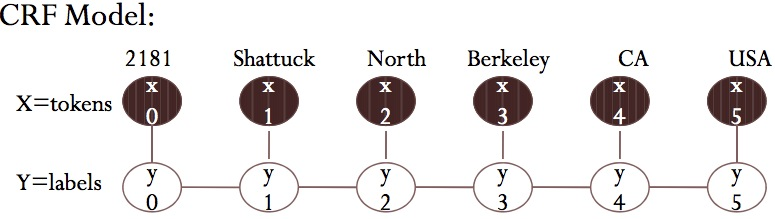
\includegraphics[height=9em]{images/crf}\\
\end{center}		             

\centering
\fbox{%
        \parbox{0.95\linewidth}{%
1.Evaluate the log-likelihood function and gradient vector for doc. $k$\\
$\ell_{\lambda_k}=\lambda F(y_k,x_k)-\log Z_\lambda(x_k)$;
$\nabla \ell_{\lambda_k}=\lambda F(y_k,x_k)-E_{p\lambda(Y|x_k)}F(Y,x_k)$\\
2.Sum up over all documents \\
$\ell_\lambda=\sum_k\ell_{\lambda_k}-\frac{\lambda^2}{2\sigma ^2}+const$;
$\nabla \ell_\lambda=\sum_k\nabla \ell_{\lambda_k}-\frac{\lambda}{\sigma ^2}$\\
3.Perform LBFGS optimization, a variation of quasi-Newton algorithm\\
$lbfgs(\lambda,\ell_\lambda,\nabla \ell_\lambda,Hessian,other args)$\\
4.Repeat step 1 and step2 until stop condition is satisfied
        }%
}\\
\fbox{%
        \parbox{0.95\linewidth}{%
\textcolor{blue}{\bf $\bf Q_1$:Loading training data into database}\\
$select$ $crf\_train\_data('/path/to/trainingdataset')$
        }%
}\\
\fbox{%
        \parbox{0.95\linewidth}{%
\textcolor{blue}{\bf $\bf Q_2$:Feature extraction for training data}\\
$select$ $crf\_train\_fgen('train\_segmenttbl', 'crf\_regex','crf\_dictionary',\\ 
'featuretbl','crf\_feature\_dic')$
        }%
}\\
\fbox{%
        \parbox{0.95\linewidth}{%
\textcolor{blue}{\bf $\bf Q_3$:Convex optimaization using LBFGS}\\
$select$ $lincrf('featuretbl','sparse\_r','dense\_m','sparse\_m','f\_size',45, \\
'crf\_feature\_dic','crf\_feature',20)$
        }%
}\\


  \end{multicols}
		 
		 }
		%%%%%%%%%%%%%%%%%%%%%%%%%%%%%%%%%%%%%%%%%%%%%%%%%%%%%%%%%%%%%%%%%%%%%%%%%%%%%%%
				%%%%%%%%%%%%%%%%%%%%%%%%%%%%%%%%%%%%%%%%%%%%%%%%%%%%%%%%%%%%%%%%%%%%%%%%%%%%%%%
		\headerbox{Parallel Viterbi Inference}{name=mycer,column=1,span=3,below=myapproxstrmatch}{
		%%%%%%%%%%%%%%%%%%%%%%%%%%%%%%%%%%%%%%%%%%%%%%%%%%%%%%%%%%%%%%%%%%%%%%%%%%%%%%%
  \begin{multicols}{2}

The Viterbi algorithm is the popular algorithm to find the top-k most likely labelings of a document 
for CRF models. 
We chose to implement a Python UDF that uses iterations to drive the Viterbi inference. Each iteration will 
finish the inference over one document.
In Greenplum, Viterbi can be run in parallel over different subsets 
of the document on a multi-core machine.
\begin{center}		             
      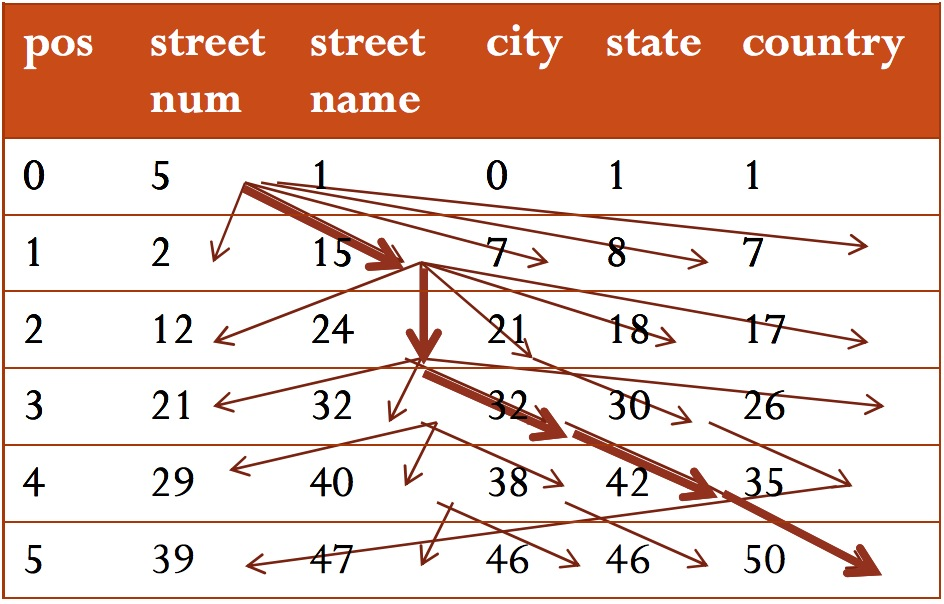
\includegraphics[height=8em,width=14em]{images/viterbip}
      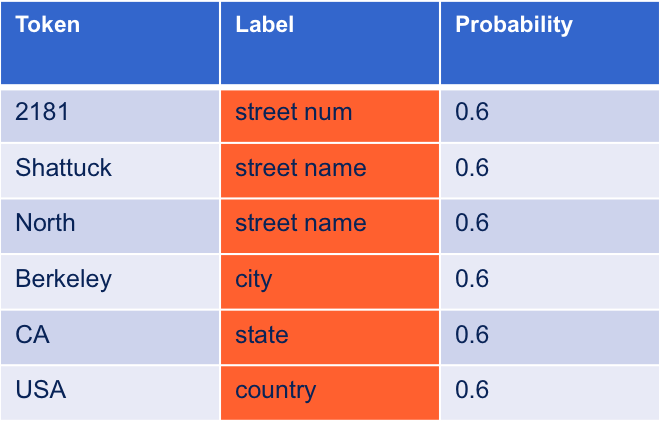
\includegraphics[height=8em,width=14em]{images/result.png}\\
\end{center}	

\centering
\fbox{%
        \parbox{0.95\linewidth}{%
$
V(i,y) =
\begin{cases}
 \max_{y^\prime}(V(i-1,y^\prime)) + \textstyle \sum_{k=1}^K \lambda_kf_k(y,y^\prime,x_i), & \text{if } i\ge0 \\
 0, & \text{if } i=-1.
\end{cases}
$
        }%
}

\fbox{%
        \parbox{0.95\linewidth}{%
\textcolor{blue}{\bf $\bf Q_4$:Loading testing data into database}\\
$select$ $crf\_test\_data('/path/to/testingdataset')$
        }%
}\\
\fbox{%
        \parbox{0.95\linewidth}{%
\textcolor{blue}{\bf $\bf Q_{5}$:Feature extraction for testing data }\\
$select$ $crf\_test\_fgen('test\_segmenttbl','crf\_dictionary','crf\_label',\\
'crf\_regex',' crf\_feature','viterbi\_mtbl','viterbi\_rtbl')$
        }%
}\\
\fbox{%
        \parbox{0.95\linewidth}{%
\textcolor{blue}{\bf $\bf Q_{6}$:TOP1 viterbi inference}\\
$select$ $vcrf\_label('test\_segmenttbl', 'viterbi\_mtbl','viterbi\_rtbl',\\ 
                 'crf\_label', 'extraction')$
        }%
}\\

  \end{multicols}

		}
		%%%%%%%%%%%%%%%%%%%%%%%%%%%%%%%%%%%%%%%%%%%%%%%%%%%%%%%%%%%%%%%%%%%%%%%%%%%%%%
		  \headerbox{Acknowledgements}{name=myacknowledgements,column=1,span=3,below=mycer} {
		%%%%%%%%%%%%%%%%%%%%%%%%%%%%%%%%%%%%%%%%%%%%%%%%%%%%%%%%%%%%%%%%%%%%%%%%%%%%%%
		  %	  \includegraphics[width=0.85\linewidth]{T-labs-Drawing-1} 
%			  \newcommand{\compactlist}{\setlength{\itemsep}{0pt} \setlength{\parskip}{0pt} \setlength{\leftskip}{-1em}}

Christan Grant is funded by a National
Science Foundation Graduate Research Fellowship under Grant No. DGE-0802270.
This work was supported by a gift from EMC Greenplum.
Thanks to C. Welton and H. Harada's code review, S. Sarawagi's work on a CRF package and N. Okazaki's work on a LBFGS implementation.
See \url{http://dsr.cise.ufl.edu} for more details.
	  	}


                %%%%%%%%%%%%%%%%%%%%%%%%%%%%%%%%%%%%%%%%%%%%%%%%%%%%%%%%%%%%%%%%%%%%%%%%%%%%%%
%                  \headerbox{References}{name=myreference,column=1,span=3,below=mycer}{
                %%%%%%%%%%%%%%%%%%%%%%%%%%%%%%%%%%%%%%%%%%%%%%%%%%%%%%%%%%%%%%%%%%%%%%%%%%%%%%
%                          \newcommand{\compactlist}{\setlength{\itemsep}{0pt} \setlength{\parskip}{0pt} \setlength{\leftskip}{-1em}}

	
		\end{poster}
		
		\end{document}
